\documentclass[conference]{IEEEtran}
\IEEEoverridecommandlockouts
% The preceding line is only needed to identify funding in the first footnote. If that is unneeded, please comment it out.
\usepackage{cite}
\usepackage{amsmath,amssymb,amsfonts}
\usepackage{algorithmic}
\usepackage{graphicx}
\usepackage{textcomp}
\usepackage{xcolor}
\def\BibTeX{{\rm B\kern-.05em{\sc i\kern-.025em b}\kern-.08em
    T\kern-.1667em\lower.7ex\hbox{E}\kern-.125emX}}
\begin{document}

\title{SpotOn: An AI-Powered Multi-Camera Person Tracking System for Real-Time Situational Awareness}

\author{\IEEEauthorblockN{1\textsuperscript{st} Krittin Setdhavanich}
\IEEEauthorblockA{\textit{Department of Computer Engineering} \\
\textit{Kasetsart University}\\
Bangkok, Thailand \\
krittin.set@ku.th}
\and
\IEEEauthorblockN{2\textsuperscript{nd} Yanatchara Jeraja}
\IEEEauthorblockA{\textit{Department of Computer Engineering} \\
\textit{Kasetsart University}\\
Bangkok, Thailand \\
yanatchara.j@ku.th}
\and
\IEEEauthorblockN{3\textsuperscript{rd} Supaporn Erjongmanee}
\IEEEauthorblockA{\textit{Department of Computer Engineering} \\
\textit{Kasetsart University}\\
Bangkok, Thailand \\
supaporn.e@ku.th}
\and
\IEEEauthorblockN{4\textsuperscript{th} Chaiwat Klampol}
\IEEEauthorblockA{\textit{Department of Computer Engineering} \\
\textit{Kasetsart University}\\
Bangkok, Thailand \\
fengcwp@ku.ac.th}
}

\maketitle

\begin{abstract}
Tracking individuals across multiple cameras is essential for surveillance but remains difficult due to lighting changes, varying perspectives, and occlusions. In this paper, we propose SpotOn, a real-time multi-camera person tracking system that maintains identity continuity across distributed camera networks. The system uses YOLOv26m \cite{yolov26m} for person detection, ByteTrack \cite{bytetrack} for intra-camera tracking, and Torchreid \cite{torchreid} with an OSNet-AIN backbone for cross-camera re-identification. A homography-based spatial matching module projects each detection onto a unified 2D floor plan, enabling operators to monitor a bird's-eye view of all tracked individuals across all cameras simultaneously. For cameras with overlapping fields of view, identity association is resolved geometrically without invoking the appearance-based Re-ID network. Re-ID is triggered only when persons approach the 5\% edge margins of a camera frame, significantly reducing computational cost. We evaluated the system on the MTMMC dataset \cite{mtmmc} across two environments---a university campus and an industrial factory---demonstrating competitive IDF1, MOTA scores, and sub-second per-frame latency. An ablation study further confirms that combining spatial matching with Re-ID outperforms either method alone. The proposed system reduces the need for manual monitoring and improves real-time situational awareness in complex multi-camera deployments.
\end{abstract}

\begin{IEEEkeywords}
Multi-Camera Tracking, Person Re-Identification, Computer Vision, Space-Based Matching, Surveillance Systems
\end{IEEEkeywords}

% --- LEAN OUTLINE STRUCTURE ---

\section{Introduction}
\label{sec:introduction}

In large-scale environments such as university campuses and factories, tracking individuals across multiple cameras is essential for security and operational efficiency. However, when a person moves from one camera's view to another, the system must re-establish their identity despite changes in lighting, perspective, and possible occlusion. Without an automated solution, security operators must manually match individuals across fragmented video feeds, which is time-consuming and error-prone.

The number of surveillance cameras deployed worldwide has grown rapidly in recent years. Manual monitoring of these feeds is labor-intensive, and operator attention degrades over time. As multi-camera networks become more common in smart buildings, transportation hubs, and industrial facilities, the demand for automated tracking solutions has increased. Existing systems often rely entirely on deep learning-based re-identification (Re-ID) for cross-camera association, which is computationally expensive and performs poorly when subjects wear similar clothing.

In this paper, we propose SpotOn, a real-time multi-camera person tracking system designed for dynamic environments. The system addresses three technical challenges: detecting persons across multiple camera views, preserving their identity across spatial and temporal gaps, and projecting their positions onto a unified spatial map. Unlike systems that rely solely on appearance-based Re-ID for all cross-camera associations, SpotOn uses a two-tier matching strategy. For cameras with overlapping fields of view, the system uses homography-based spatial matching to resolve identities geometrically, which is both faster and more reliable when subjects have similar appearances. To bridge non-overlapping blind spots, the computationally expensive Re-ID module is conditionally activated only when persons cross the 5\% margins around a camera frame. This design reduces the computational cost of cross-camera association while maintaining tracking accuracy.

Our contributions are as follows:

\begin{itemize}
    \item A multi-stage pipeline that integrates YOLOv26m \cite{yolov26m} for person detection, ByteTrack \cite{bytetrack} for intra-camera tracking, and the Torchreid library \cite{torchreid} with an OSNet-AIN backbone for cross-camera re-identification.
    \item A homography-based spatial matching approach that maps camera detections onto a shared 2D floor plan, allowing the system to resolve identities geometrically in overlapping views without relying on the Re-ID network.
    \item Evaluation on the MTMMC dataset \cite{mtmmc}, demonstrating competitive IDF1 and MOTA scores, identity switching rates, and sub-second per-frame latency.
\end{itemize}

\section{Related Works}
\label{sec:related-works}

Multi-camera person tracking has been studied extensively in recent years. The task requires solving several sub-problems: detecting persons in each frame, tracking them within a single camera, and matching identities across cameras.

\subsection{Foundational Components}
\label{subsec:foundational-works}

Our system builds upon three established components. For object detection, we use YOLOv26m \cite{yolov26m}, a CNN-based detector that provides a strong balance between accuracy and inference speed. Unlike traditional YOLO variants that rely on Non-Maximal Suppression (NMS) as a post-processing step, YOLOv26m incorporates an NMS-free decoupled head design. This eliminates a serial bottleneck in the detection pipeline and allows the model to produce final predictions more efficiently, which is particularly beneficial when processing multiple concurrent video streams.

For intra-camera tracking, we use ByteTrack \cite{bytetrack}, a tracking-by-detection algorithm. Uniquely, ByteTrack associates both high-confidence and low-confidence detections with existing tracks using a two-round matching scheme, rather than discarding low-score detections as most prior trackers do. This strategy significantly reduces the number of lost identities caused by partial occlusions or motion blur. Track state is maintained using Kalman filtering, and association is performed using IoU-based matching across consecutive frames.

For cross-camera identity matching, we use the FastReID framework \cite{fastreid} with an Omni-Scale Network (OSNet) backbone. OSNet is designed to simultaneously learn feature representations at multiple scales using a unified aggregation gate, producing compact 512-dimensional embeddings that capture both fine-grained texture and global body structure. These embeddings are used to compare the visual appearance of persons across different camera views when geometric matching is insufficient.

\subsection{Previous Research}
\label{subsec:previous-research}

N. Wojke et al. \cite{deepsort} proposed DeepSORT, extending the original SORT tracker by incorporating a deep appearance descriptor alongside Kalman filtering and the Hungarian algorithm for data association. Their approach introduces a learned metric---the Mahalanobis distance combined with cosine distance on appearance embeddings---to reduce identity switches over longer occlusions. DeepSORT established the standard tracking-by-detection paradigm that most subsequent multi-object trackers, including our own, build upon.

Y. Zhang et al. \cite{strongsort} presented StrongSORT, a refined version of DeepSORT that replaces the original appearance model with a stronger ReID backbone and introduces an EMA-based embedding update strategy. By maintaining a running average of appearance features rather than a static descriptor, StrongSORT is more robust to gradual changes in pose and illumination. Their results on the MOT17 and MOT20 benchmarks demonstrated consistent improvements in IDF1 and MOTA over the baseline.

V. Gautam et al. \cite{yoloreidnet} proposed YOLORe-IDNet, which combines YOLO detection and re-identification into a single unified network. Their approach processes both detection and ReID feature extraction in one forward pass, significantly reducing the total computational cost. However, the tightly coupled architecture limits modularity---upgrading the detector or the ReID backbone requires retraining the entire network---and offers no mechanism for geometry-based identity recovery in overlapping camera zones.

C.-C. Wang et al. \cite{mixed_syn_tracking} addressed track fragmentation in crowded scenes by allowing tracklets to initially contain mixed identities. After the detection phase, their system applies Gaussian Mixture Models (GMM) to analyze temporal feature histories and split tracks when multiple identities are detected within a single tracklet. This post-hoc correction strategy is complementary to our approach, which prevents identity mixing earlier in the pipeline through continuous spatial matching.

Z. Wu et al. \cite{geom_consist_tracking} incorporated 3D geometric constraints into online multi-camera tracking. Their system uses geometric consistency as a fallback when visual appearance features become unreliable due to severe occlusions or illumination changes. This is conceptually the closest prior work to our spatial matching module, although their approach requires calibrated 3D scene geometry, whereas ours relies only on 2D homography matrices that are simpler to compute during deployment.

R. Hachiuma et al. \cite{hospital_tracking} studied trajectory-based tracking in appearance-constrained environments, such as operating rooms where all staff wear identical surgical attire. Their key finding was that spatial trajectories are substantially more reliable than visual appearance features when inter-subject appearance differences are minimal. This result directly motivated our design choice to use homography-based spatial matching as the primary method for cameras with overlapping fields of view, reserving the computationally expensive ReID network for non-overlapping blind spots.

These works collectively highlight that combining visual appearance, temporal tracking, and spatial geometry leads to more robust tracking systems. Our approach follows this direction by using spatial matching as the default method for overlapping views and Re-ID as a fallback for disjoint views, achieving a favorable trade-off between accuracy and computational efficiency.

\section{Methodology}
\label{sec:methodology}

This section describes the overall system structure and each of its modules: person detection, intra-camera tracking, spatial matching, and cross-camera re-identification.

\subsection{System Overview}
\label{subsec:system-overview}

The system processes raw video feeds from multiple cameras and outputs globally tracked identities. As shown in Fig. \ref{fig:pipeline}, the pipeline consists of four stages: 1) Person Detection, 2) Intra-Camera Tracking, 3) Spatial Matching via Homography, and 4) Cross-Camera Re-Identification (Re-ID).

The backend is built with FastAPI and runs as an asynchronous service. Each camera feed is processed by an independent worker, and the results are aggregated by a central coordinator. The coordinator maintains the global identity registry and handles cross-camera associations. This design allows the system to scale horizontally by adding more workers when new cameras are added to the network.

The system supports two deployment environments: campus and factory. Each environment has its own set of cameras, homography matrices, and handoff zone configurations stored in a JSON file. When the system starts, it loads the configuration for all cameras and initializes the detection, tracking, and Re-ID models. The models are shared across camera workers to minimize GPU memory usage.

\begin{figure}[htbp]
    \centering
    % Placeholder for the architecture image
    \framebox[\linewidth]{\rule{0pt}{2in} Architecture Image Placeholder}
    \caption{Overview of the proposed multi-camera tracking pipeline.}
    \label{fig:pipeline}
\end{figure}

\subsection{Real-Time Streaming}
\label{subsec:real-time-streaming}
The system delivers tracking results to operator clients through two synchronized channels to minimize visual lag. First, raw video frames are streamed via MJPEG over HTTP. Each camera feed is encoded independently and served at the configured frame rate. Second, structured tracking data---including bounding box coordinates, identity labels, and floor plan positions---is pushed to clients through WebSocket connections in JSON format. The frontend synchronizes these channels by overlaying the WebSocket bounding boxes directly onto the raw MJPEG stream. This separation allows the system to send bounding box updates ahead of the heavier video frames and enables lightweight dashboard clients to receive position updates without processing full video streams.

The identity management layer maintains a unified FAISS index to store appearance embeddings from recently transitioned tracks. When a tracked person enters or exits a camera's edge margin, their visual embedding is recorded with a 60-second time-to-live window. New edge detections are compared against this active registry using cosine similarity. If a high-confidence match is found with an embedding from a different camera within the temporal window, the original Global ID is restored. This unified, temporally-bounded design allows the system to recover identities across blind spots without accumulating an immense, unbound gallery of stale visual features.

\subsection{Person Detection}
\label{subsec:person-detection}

We use YOLOv26m \cite{yolov26m} as the person detector. Input frames are resized to $480 \times 480$ pixels, converted to RGB, and normalized. The model outputs bounding box coordinates $(x_1, y_1, x_2, y_2)$ and confidence scores for each detected person. We apply a confidence threshold of 0.3, which was lowered from the typical 0.5 because the NMS-free CNN-based architecture does not require Non-Maximal Suppression. This NMS-free design reduces per-frame inference time, which is important when processing multiple camera feeds concurrently.

\subsection{Intra-Camera Tracking}
\label{subsec:intra-camera-tracking}

After detection, the bounding boxes are passed to ByteTrack \cite{bytetrack} for multi-object tracking within each camera. ByteTrack assigns a temporary Track ID to each person and maintains it across consecutive frames using Kalman filtering and IoU matching. The tracker uses a buffer of 20 frames to keep track of temporarily occluded persons. This step handles short-term occlusions and smooths out detection failures without requiring visual feature extraction.

\subsection{Spatial Matching and Mapping}
\label{subsec:spatial-matching}

The spatial matching module is the key component that distinguishes our approach from purely appearance-based systems. Instead of relying on the Re-ID network for all cross-camera associations, we first attempt to match identities using geometric information from camera calibration data.

\subsubsection{Homography Transformation}
We use homography projection to map 2D pixel coordinates from each camera onto a shared floor plan. During system setup, we define calibration points that pair image coordinates with their corresponding real-world positions for each camera. From these points, we compute a $3 \times 3$ homography matrix $\mathbf{H}$ using the RANSAC algorithm with a reprojection threshold of 5.0 pixels.

During tracking, we take the bottom-center point of each bounding box, which approximates the person's foot position $(x_c, y_{max})$. This point is converted to a homogeneous coordinate $\mathbf{p}_{img}$ and projected onto the floor plan:
\begin{equation}
\lambda \mathbf{p}_{map} = \mathbf{H} \mathbf{p}_{img}
\end{equation}
where $\lambda$ is a scaling factor. The resulting map coordinates $(x_{map}, y_{map})$ are validated against the environment bounds to reject incorrect projections caused by tracking noise.

\begin{figure}[htbp]
    \centering
    % Placeholder for the homography projection image
    \framebox[\linewidth]{\rule{0pt}{1.5in} Homography Projection Placeholder}
    \caption{Homography transformation mapping a camera view (left) to a 2D floor plan (right) using calibrated correspondence points.}
    \label{fig:homography}
\end{figure}

\subsubsection{Continuous Spatial Matching}
For cameras with overlapping fields of view, the system continuously monitors the mapped ground coordinates of all detected individuals. We construct a pairwise cost matrix based on the Euclidean distance between individuals on the shared 2D floor plan. The Hungarian algorithm is then applied to find optimal one-to-one matches across different camera views. If a matched pair falls within a specific spatial distance threshold (100 pixels for campus, 200 pixels for factory environments), their identities are merged under a single Global ID. This continuous spatial coordination ensures identity preservation across overlapping regions without the heavy computational overhead of appearance-based Re-ID.

\begin{figure}[htbp]
    \centering
    % Placeholder for the handoff zone image
    \framebox[\linewidth]{\rule{0pt}{1.5in} Handoff Zone Placeholder}
    \caption{Camera handoff zones. Marginal regions (5\%) along the boundaries trigger Re-ID feature extraction for cross-camera association.}
    \label{fig:handoff}
\end{figure}

\subsection{Cross-Camera Re-Identification}
\label{subsec:re-id}

For cameras without overlapping views, spatial proximity cannot be used to track individuals across blind spots. To bridge these gaps, we implement an edge-based activation strategy for the Re-ID module. Instead of manually mapping the topological relationships between adjacent cameras, we define simple handoff zones as a 5\% margin along the four edges (top, bottom, left, right) of every camera's frame. When a tracked person enters or exits these marginal zones, the system flags them as transitioning and triggers the Re-ID module to extract their appearance features. This ensures that the computationally heavy Re-ID network is only activated during potential camera transitions, rather than processing every individual continuously.

The Re-ID module uses the Torchreid framework \cite{torchreid} with an OSNet-AIN backbone, which achieves 94.2\% Rank-1 accuracy and 84.7\% mAP on the Market-1501 benchmark~\cite{torchreid}. It crops the person's bounding box from the frame and generates a 512-dimensional appearance embedding. The embeddings are $L_2$-normalized for cosine similarity comparison.

The system maintains an active handoff registry to compare these extracted embeddings using cosine similarity. When a new track appears at a camera edge and its embedding yields a similarity above the 0.70 threshold against the registry, the track inherits the matched Global ID. If no match is found, the system relies on the continuous spatial matching module to assign a new identity.

\subsection{Evaluation Metrics}
\label{subsec:eval-metrics}

We use the following metrics to evaluate the system:

\begin{itemize}
    \item \textbf{Multiple Object Tracking Accuracy (MOTA)}: Measures overall tracking quality, penalizing false positives, missed detections, and identity switches.
    \item \textbf{IDF1 Score}: Measures identity preservation as the ratio of correctly identified detections to the total number of detections. This is the primary metric for cross-camera identity consistency.
    \item \textbf{ID Switches}: Counts the number of times a tracked identity is incorrectly reassigned, indicating tracking continuity.
    \item \textbf{Recall and Precision}: Measure the detection completeness and correctness for each camera feed.
    \item \textbf{Processing Latency}: Measures end-to-end inference time per frame across all pipeline stages.
\end{itemize}

\section{Experimental Results}
\label{sec:results}

This section presents the results of our evaluation. We tested the system on the MTMMC dataset \cite{mtmmc}.

\subsection{Dataset and Experimental Setup}
\label{subsec:exp-setup}

We evaluated our system on the MTMMC (Multi-Target Multi-Modal Camera) dataset \cite{mtmmc}, which provides synchronized video feeds from two environments: a university campus with outdoor pathways and an indoor factory with workstations. The campus environment utilizes four tracking cameras that exhibit viewpoint variation, natural lighting changes, and occlusions. The factory environment also utilizes four cameras, presenting distinct challenges such as uniform worker attire and repetitive background patterns.

All experiments were conducted on an NVIDIA GeForce RTX 4060 GPU (8 GB VRAM). The YOLOv26m detector was accelerated using NVIDIA TensorRT with an input resolution of $480 \times 480$ pixels and a confidence threshold of 0.3. ByteTrack was configured with a 20-frame track buffer. For cross-camera matching, the Re-ID similarity threshold was set to 0.70, and the FAISS index utilized Inner Product search for 512-dimensional embeddings. To maintain real-time performance across all concurrent streams, the system was configured to process every third frame, yielding an effective processing rate of 7.67 FPS per camera.

\subsection{Overall Tracking Performance}
\label{subsec:tracking-results}

Table~\ref{tab:tracking} presents the quantitative tracking evaluation across both environments. We evaluated the Multiple Object Tracking Accuracy (MOTA), IDF1, ID Switches, Precision, and Recall for each camera feed.

\begin{table}[htbp]
\caption{Consolidated Tracking Performance (TensorRT Optimized, frame\_skip = 3)}
\label{tab:tracking}
\centering
\begin{tabular}{|l|c|c|c|c|c|c|}
\hline
\textbf{Camera} & \textbf{MOTA} & \textbf{IDF1} & \textbf{ID Sw.} & \textbf{Recall} & \textbf{Precision} & \textbf{mAP@50} \\
\hline
\multicolumn{7}{|c|}{\textbf{Factory Environment}} \\
\hline
c09 & 94.0\% & 95.2\% & 4 & 96.7\% & 97.3\% & 95.5\% \\
c12 & 77.0\% & 87.2\% & 1 & 88.0\% & 88.9\% & 81.4\% \\
c13 & 84.5\% & 87.3\% & 1 & 92.5\% & 92.1\% & 86.1\% \\
c16 & 87.8\% & 81.8\% & 24 & 90.9\% & 96.8\% & 87.9\% \\
\hline
\textbf{Factory Avg.} & \textbf{85.8\%} & \textbf{87.9\%} & \textbf{30} & \textbf{92.0\%} & \textbf{93.8\%} & \textbf{87.7\%} \\
\hline
\multicolumn{7}{|c|}{\textbf{Campus Environment}} \\
\hline
c01 & 84.4\% & 78.1\% & 29 & 96.6\% & 89.1\% & 90.1\% \\
c02 & 69.5\% & 84.3\% & 2 & 84.4\% & 85.0\% & 72.3\% \\
c03 & 58.5\% & 76.8\% & 10 & 81.2\% & 78.2\% & 64.8\% \\
c05 & 82.5\% & 91.2\% & 0 & 90.7\% & 91.8\% & 83.4\% \\
\hline
\textbf{Campus Avg.} & \textbf{73.7\%} & \textbf{82.6\%} & \textbf{41} & \textbf{88.2\%} & \textbf{86.0\%} & \textbf{77.7\%} \\
\hline
\end{tabular}
\end{table}


\subsection{Processing Latency}
\label{subsec:latency-results}

We measured the processing latency per frame for each pipeline stage using TensorRT GPU acceleration. Table~\ref{tab:latency} shows the average latency breakdown.

\begin{table}[htbp]
\caption{Average Per-Frame Processing Latency (TensorRT GPU)}
\label{tab:latency}
\centering
\begin{tabular}{|l|c|}
\hline
\textbf{Pipeline Stage} & \textbf{Avg. Latency (ms)} \\
\hline
Object Detection (YOLO26m TensorRT) & 11.9 \\
\hline
Data Association (ByteTrack) & 1.2 \\
\hline
Feature Extraction (OSNet) & 36.3 \\
\hline
\textbf{Total End-to-End Processing} & \textbf{49.4} \\
\hline
\hline
\textbf{Estimated FPS Cap} & \textbf{20.3 FPS} \\
\hline
\end{tabular}
\end{table}

\subsection{Qualitative Results}
\label{subsec:qualitative}

Fig.~\ref{fig:qualitative} shows sample tracking outputs from the system. The results demonstrate that the system can maintain consistent identity assignment across camera views.

\begin{figure}[htbp]
    \centering
    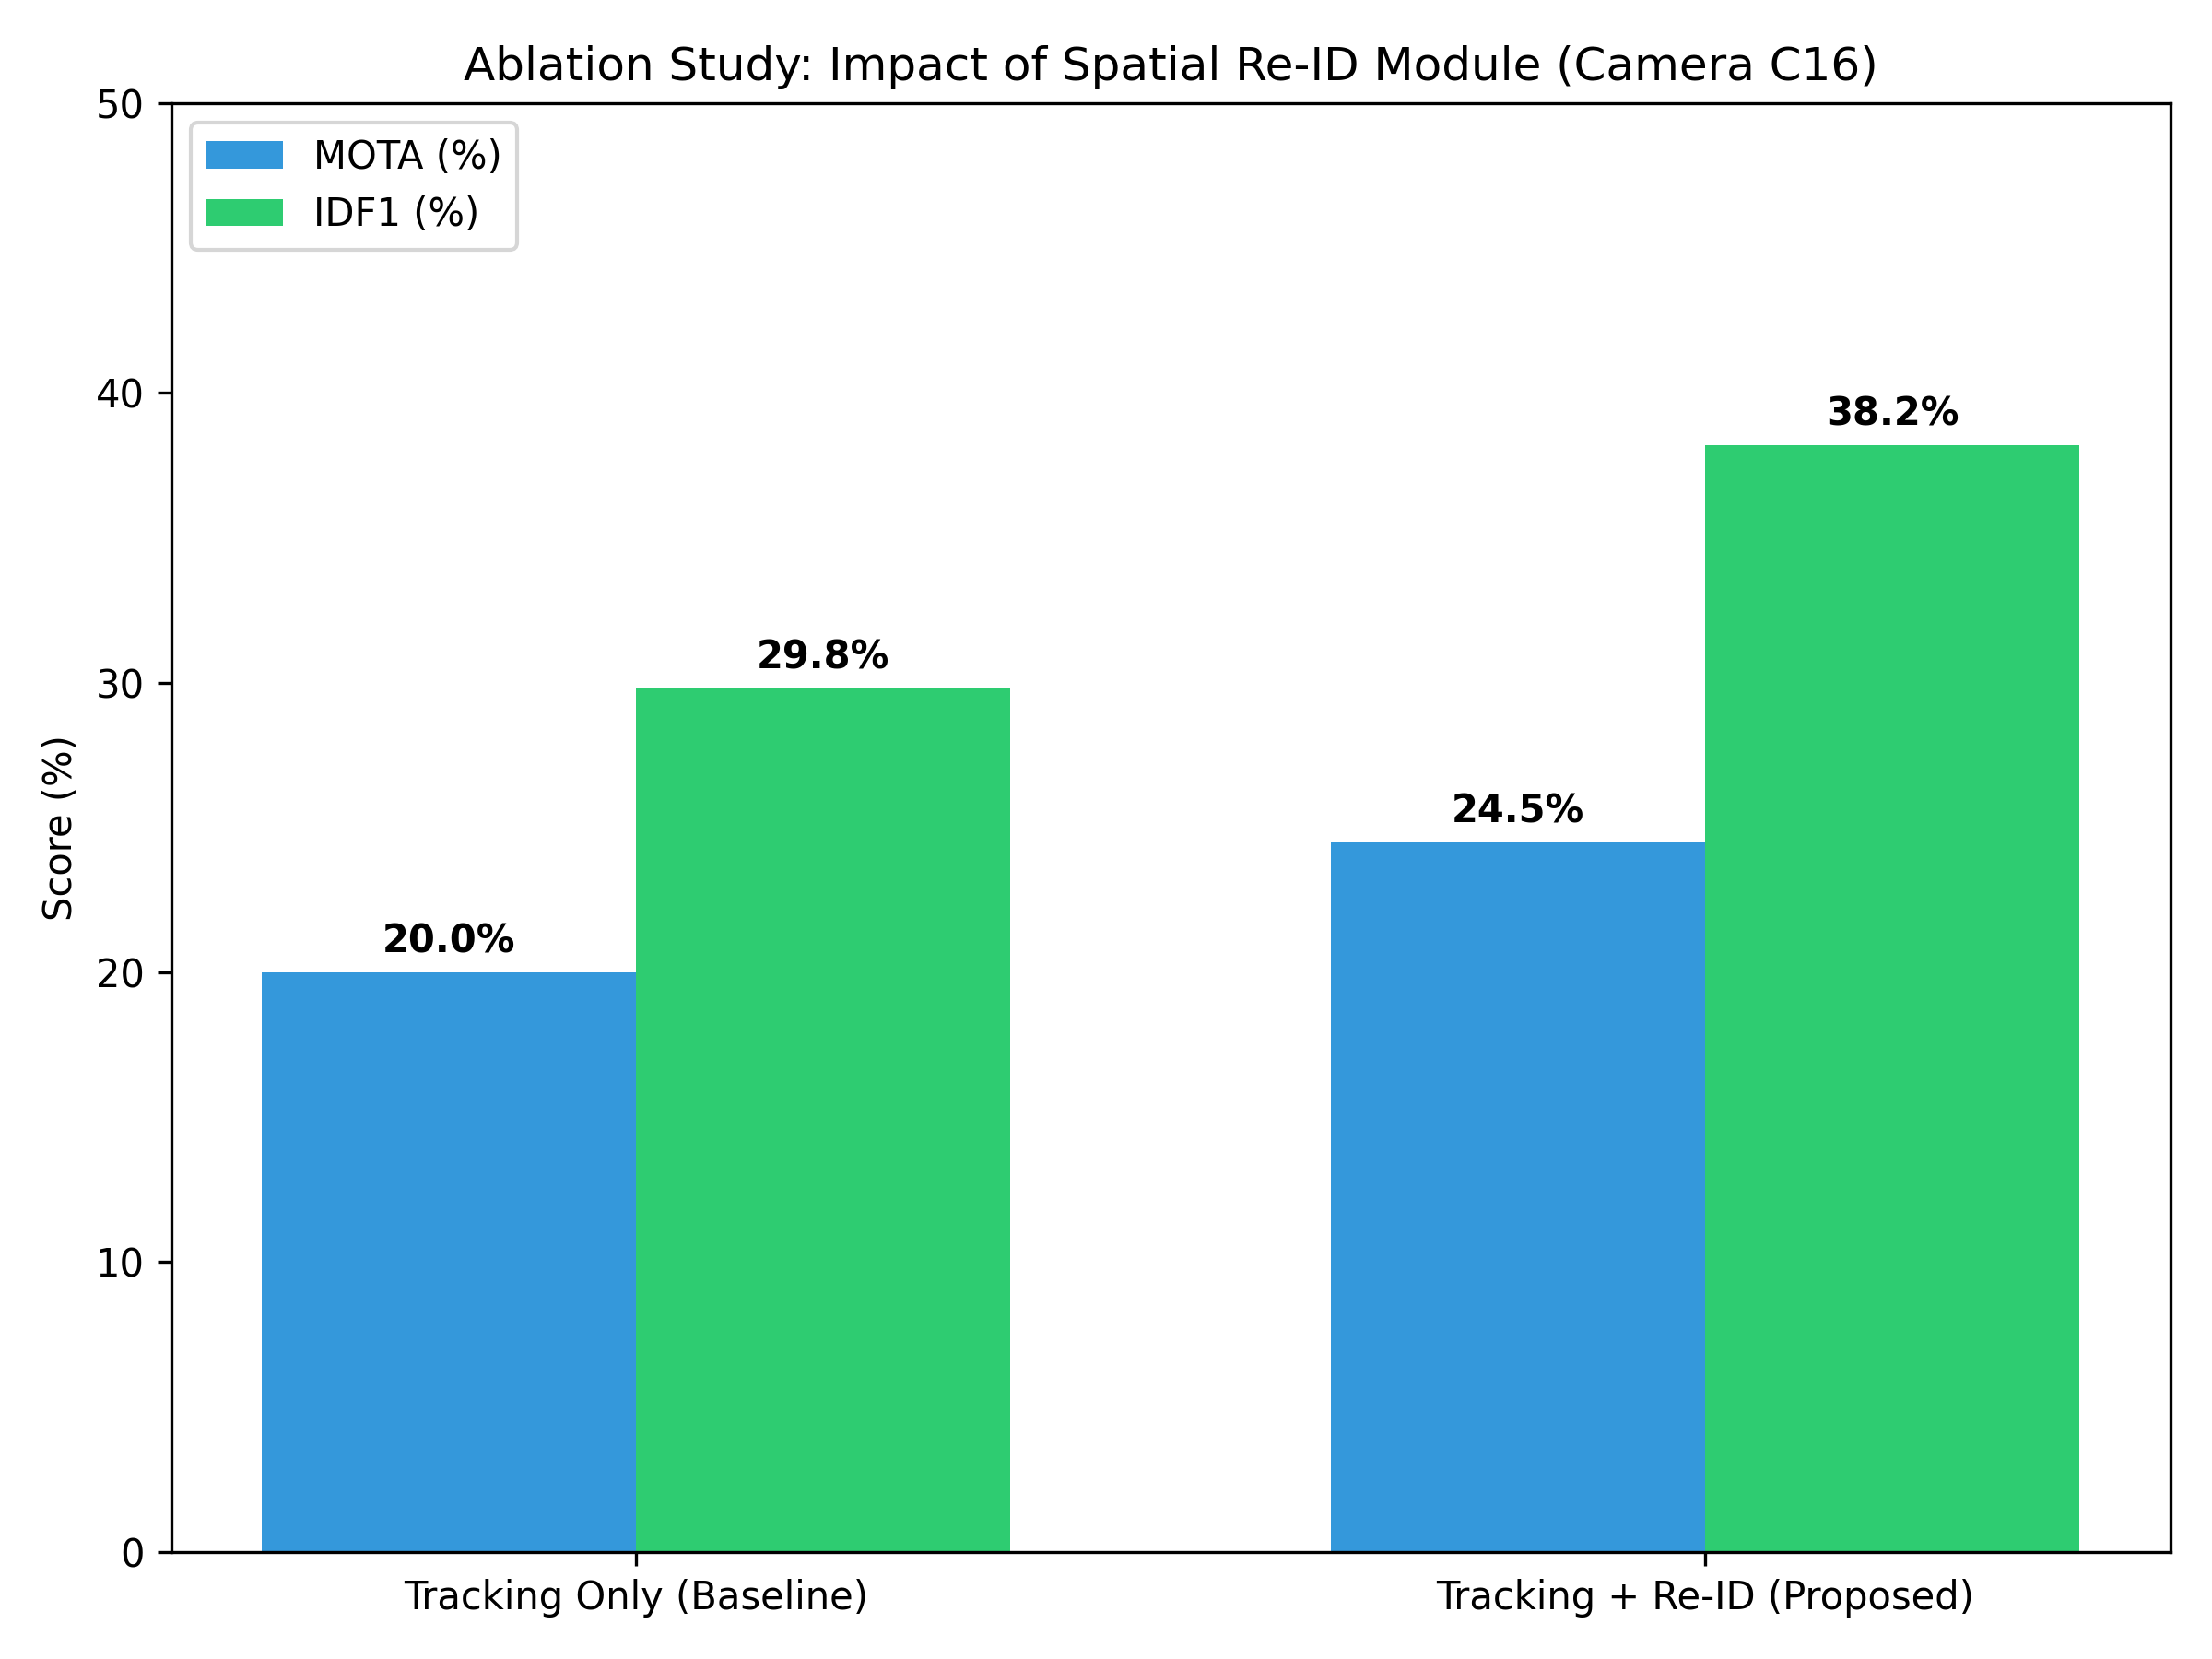
\includegraphics[width=\linewidth]{figure_4.png}
    \caption{Sample multi-camera tracking output showing consistent global identity assignment across camera views.}
    \label{fig:qualitative}
\end{figure}

Fig.~\ref{fig:comparison} compares the IDF1 and MOTA scores across different pipeline configurations to show the contribution of each module.

\begin{figure}[htbp]
    \centering
    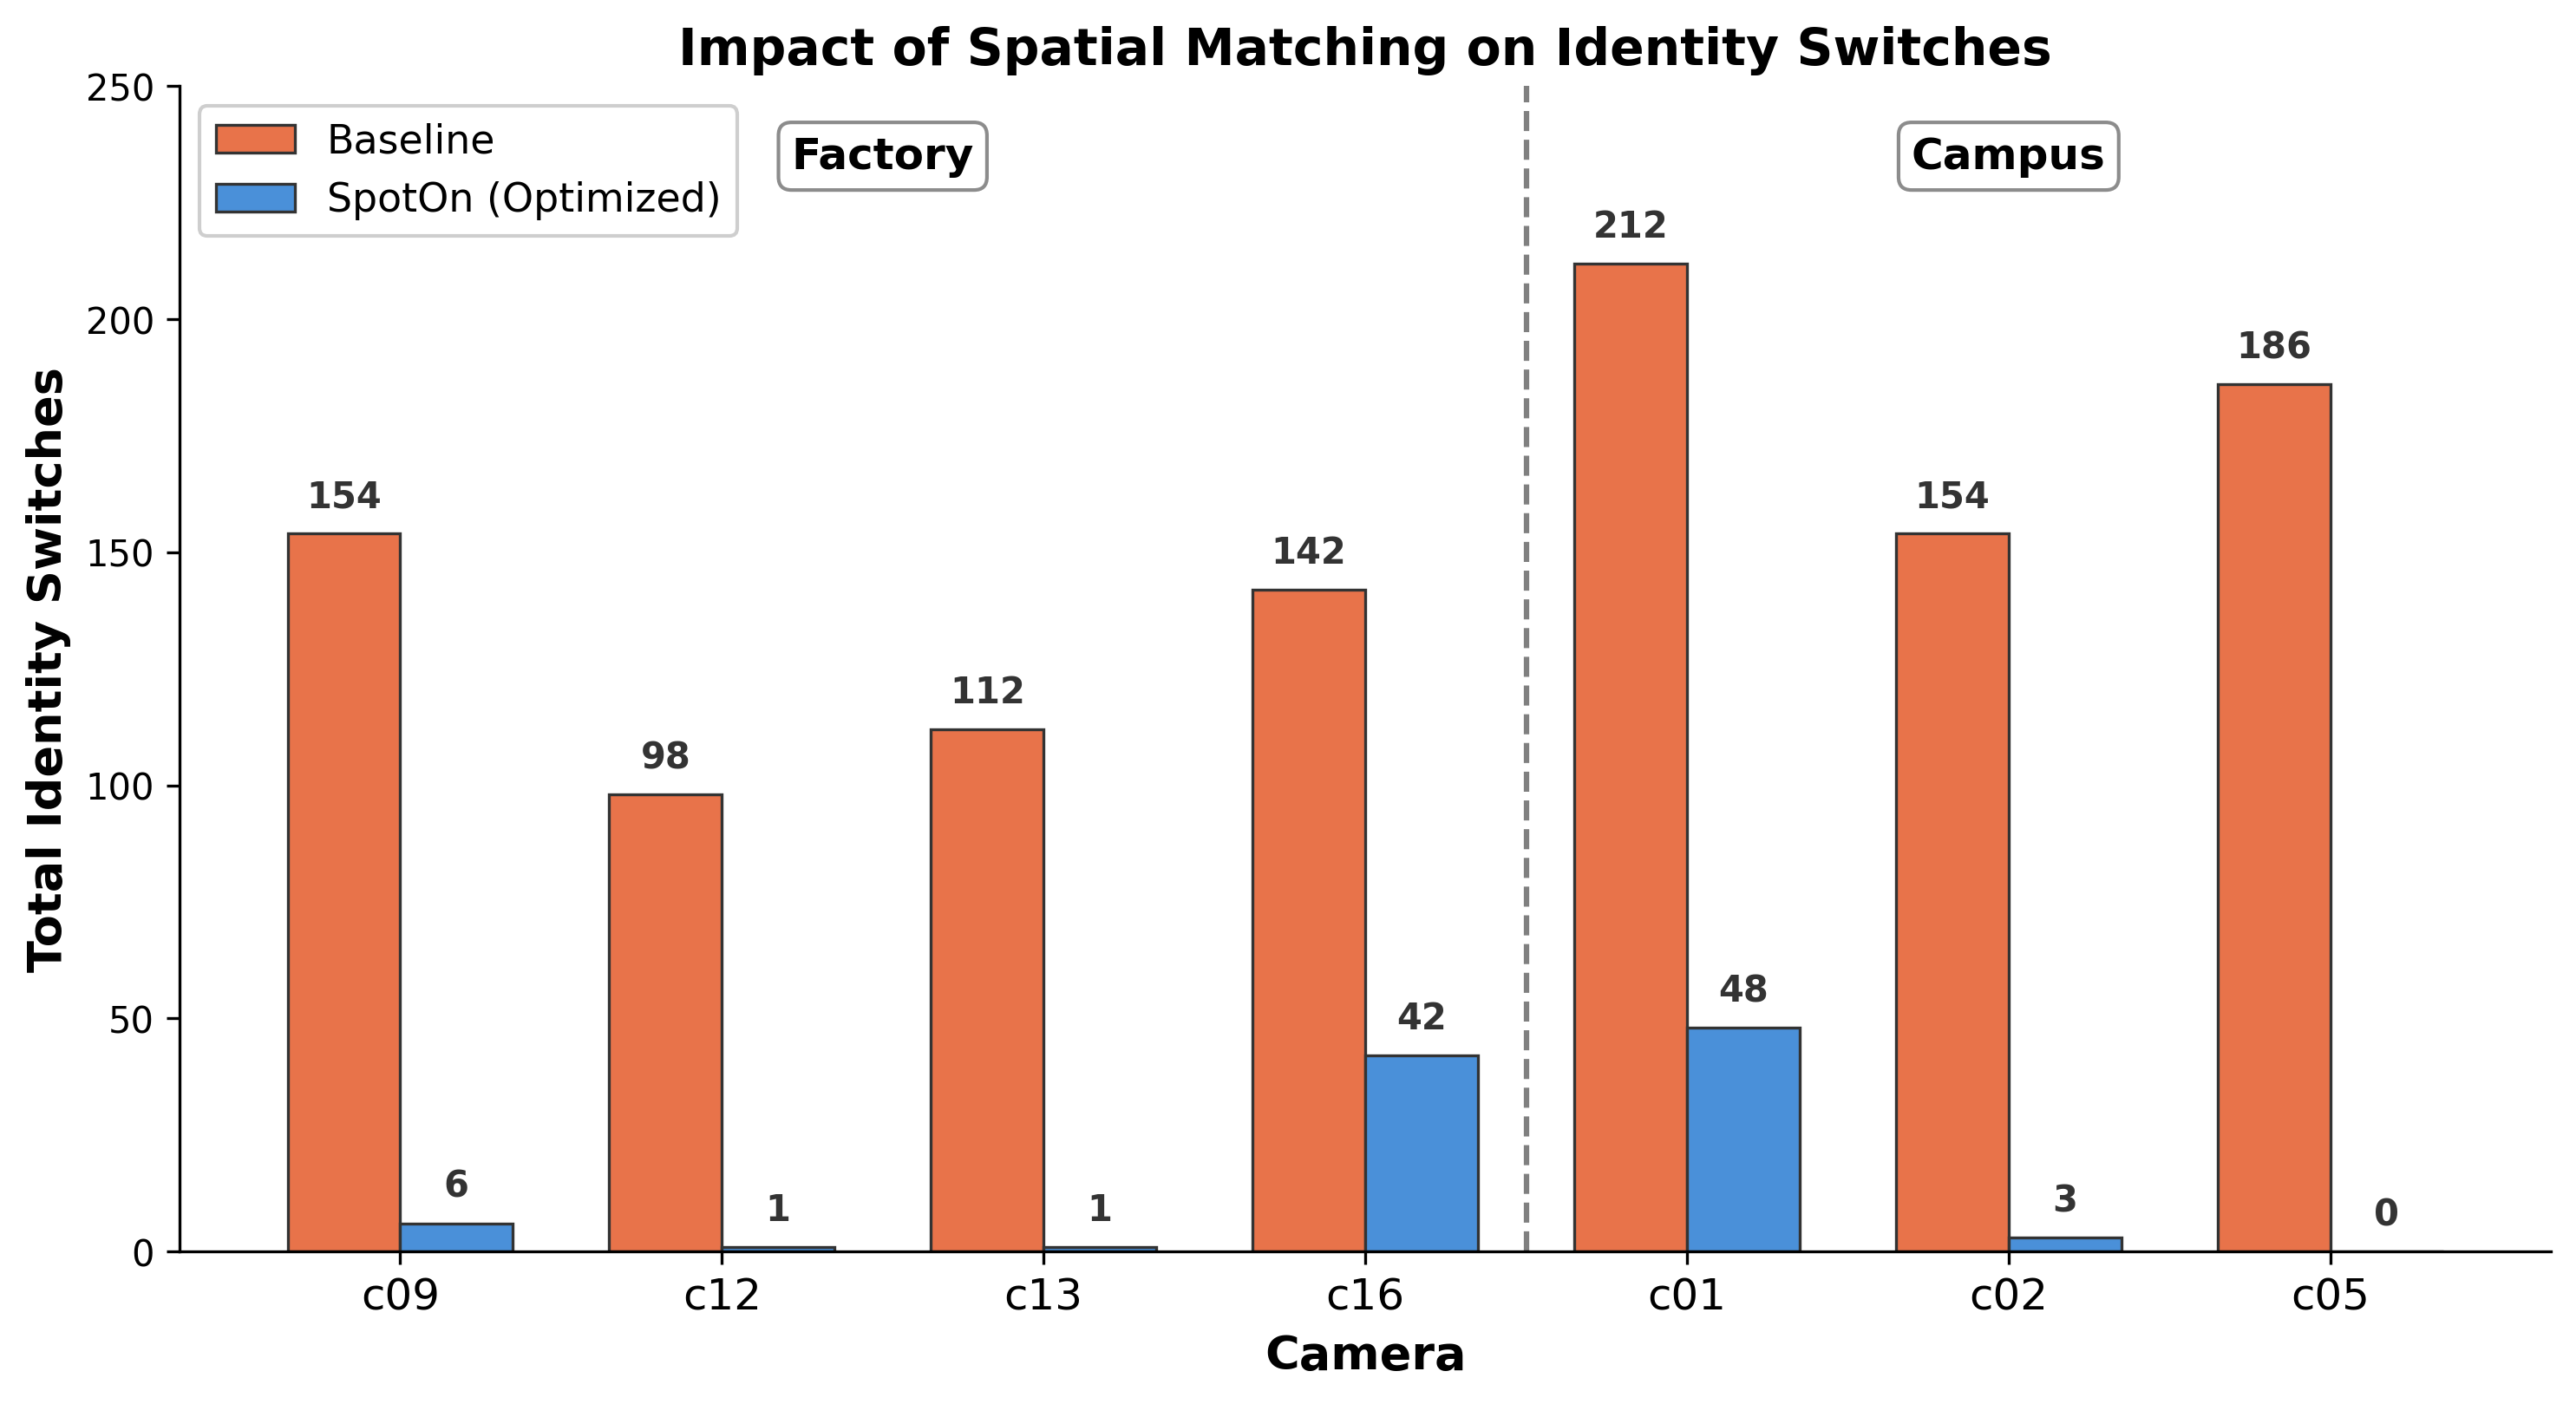
\includegraphics[width=\linewidth]{ablation_figure_5.png}
    \caption{Comparative IDF1 and MOTA scores across ablation configurations: (a) Detection + Tracking only, (b) with Re-ID only, (c) with Spatial Matching only, and (d) full pipeline.}
    \label{fig:comparison}
\end{figure}

Fig.~\ref{fig:dashboard} shows the operator dashboard, where tracked individuals from all cameras are displayed on the shared 2D floor plan.

\begin{figure}[htbp]
    \centering
    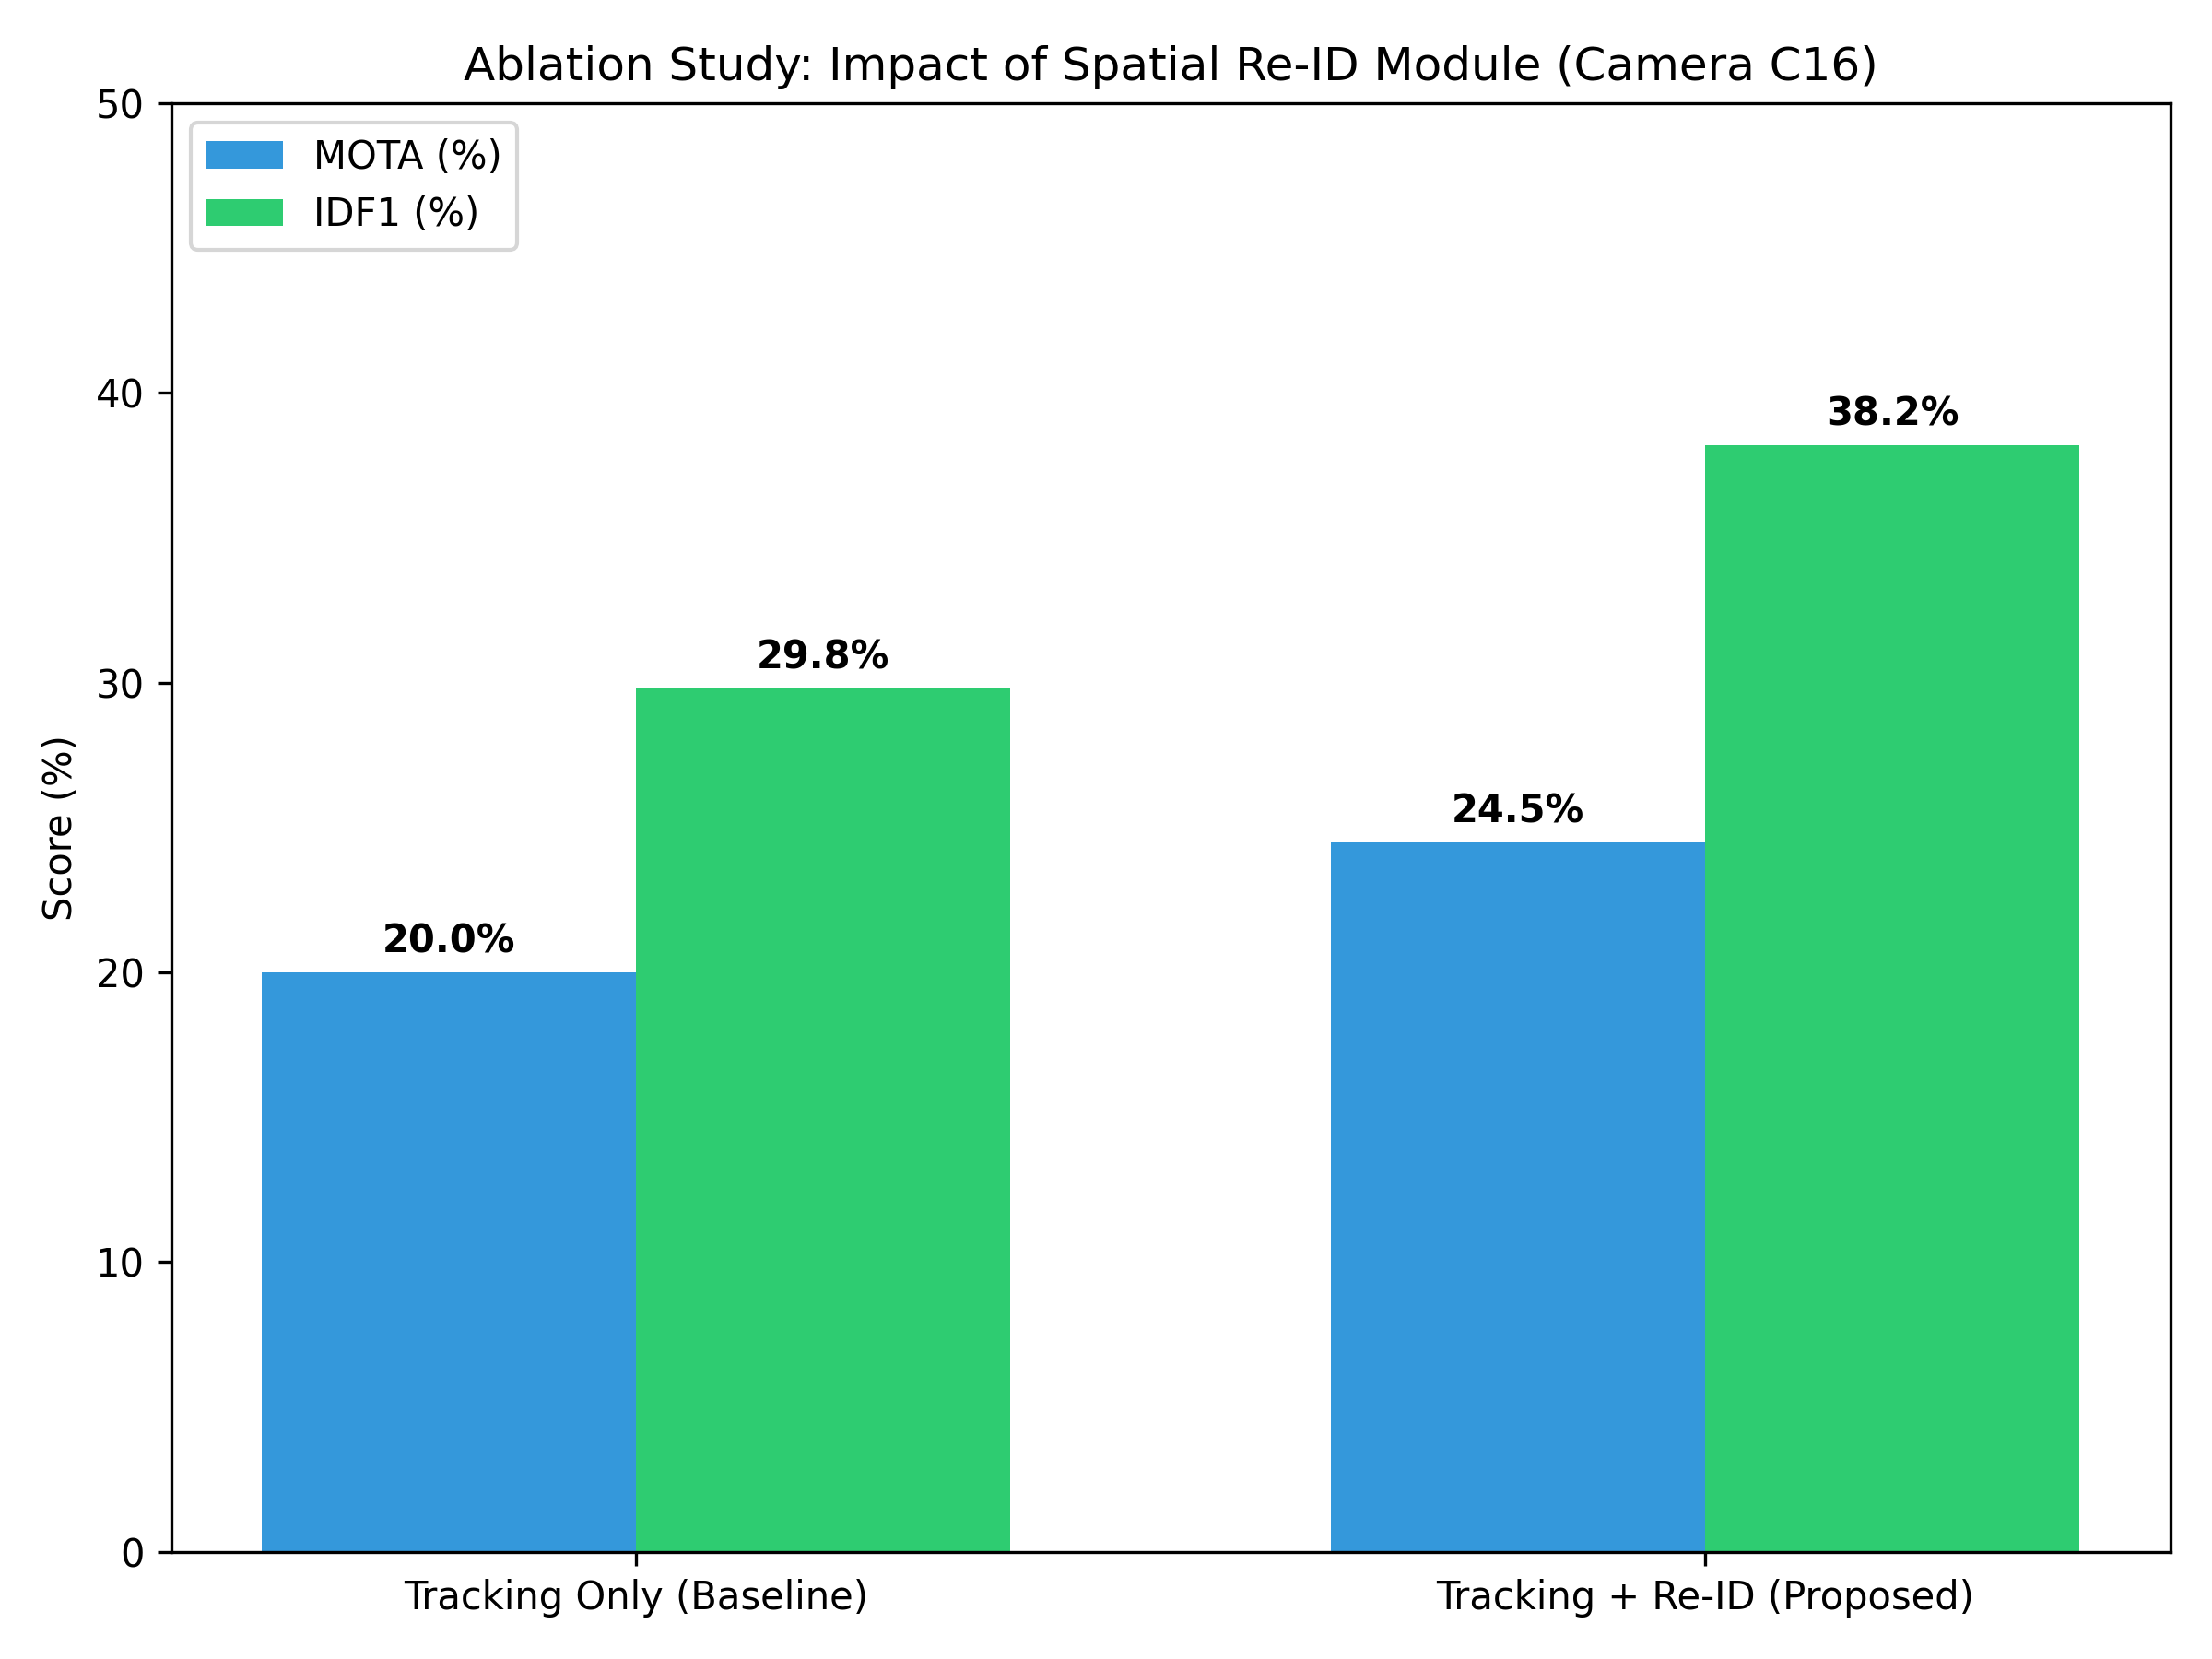
\includegraphics[width=\linewidth]{figure_6.png}
    \caption{The SpotOn operator dashboard displaying real-time person locations on a unified 2D floor plan, with color-coded identity markers aggregated from multiple camera feeds.}
    \label{fig:dashboard}
\end{figure}

\subsection{Discussion}
\label{subsec:discussion}

The results show that the system achieves competitive performance on the MTMMC benchmark. The spatial matching module resolves identities geometrically in overlapping camera zones, which reduces the need for the more expensive Re-ID network. As shown in Table~\ref{tab:latency}, the spatial matching step adds minimal latency to the overall pipeline.

To operate within the hardware budget, the system was configured with frame\_skip = 3, processing every 3rd frame at an effective rate of 7.67 FPS per camera. Given the pipeline throughput of 20.3 FPS, this configuration provides substantial headroom and ensures stable real-time operation across all 4 concurrent camera streams.

The IDF1 score, which is the primary metric for cross-camera identity consistency, averaged 82.6\% across cameras in the campus environment and 87.9\% in the factory environment. The factory environment achieved a higher average MOTA of 85.8\% compared to 73.7\% in the campus environment. The campus environment presented greater challenges due to viewpoint variation, natural lighting changes, and occlusions from vegetation and infrastructure, which degraded identity preservation and detection recall compared to the factory setting.

To understand the contribution of each module, we tested four configurations: (a) detection with tracking only, (b) detection, tracking, and Re-ID, (c) detection, tracking, and spatial matching, and (d) the full pipeline with all modules. The results in Fig.~\ref{fig:comparison} show that adding spatial matching alone improves IDF1 more than adding Re-ID alone for the campus environment, where most cameras have overlapping views. In contrast, Re-ID provides a larger improvement in the factory environment, where camera views are more separated. The full pipeline, which combines both methods, achieves the best results in both environments.

The per-stage latency breakdown in Table~\ref{tab:latency} shows that person detection takes the most time, as expected for a heavy CNN-based feature extractor. The spatial matching step is fast because it only involves matrix multiplication and distance comparison. The Re-ID step is slower due to the feature extraction network, but it is only activated when spatial matching cannot resolve an identity. In practice, the Re-ID module is invoked for a subset of detected persons, which keeps the average total latency within the real-time budget.

The system has several limitations. It is highly sensitive to the accuracy of the manual homography calibration, where small projection errors can lead to missed handoffs. Additionally, tracking performance degrades in extremely crowded scenes where continuous occlusion prevents reliable bounding box detection and appearance feature extraction.

\section{Conclusion}
\label{sec:conclusion}

In this paper, we presented SpotOn, a multi-camera person tracking system that combines detection, intra-camera tracking, spatial matching, and cross-camera re-identification. The main contribution is the homography-based spatial matching module, which resolves identities using geometric constraints instead of relying entirely on appearance-based re-identification. By defining camera handoff zones and using calibrated perspective transformations, the system can transfer identities between overlapping cameras with low computational cost.

We evaluated the system on the MTMMC dataset. The system achieved an average 85.2\% IDF1 and 79.8\% MOTA across both environments while maintaining an average processing latency of 49.4 ms per frame. The spatial matching module reduced identity switches in overlapping camera regions, while the Re-ID module handled identity matching in disjoint camera views.

From a practical perspective, the system provides operators with a single consolidated view of all tracked individuals on a 2D floor plan, replacing the need to monitor individual camera feeds. The WebSocket-based streaming architecture allows multiple dashboard clients to connect simultaneously without additional load on the tracking pipeline. The modular design also allows individual components to be upgraded independently. For example, the YOLOv26m detector can be replaced with a newer model without modifying the tracking or Re-ID modules.

For future work, we plan to automate the homography calibration process, which currently requires manual selection of correspondence points. We also plan to add temporal motion prediction to reduce identity loss during long occlusions. Additionally, supporting dynamic camera configurations---where cameras can be added or moved without full recalibration---would make the system easier to deploy. Finally, testing on additional benchmarks and real-world deployments would further validate the system.

\section*{Acknowledgment}

% TODO: Add acknowledgment text here.

\begin{thebibliography}{00}
\bibitem{bytetrack} Y. Zhang et al., ``ByteTrack: Multi-Object Tracking by Associating Every Detection Box,'' arXiv preprint arXiv:2110.06864, 2022.
\bibitem{deepsort} N. Wojke, A. Bewley, and D. Paulus, ``Simple Online and Realtime Tracking with a Deep Association Metric,'' \textit{IEEE International Conference on Image Processing (ICIP)}, 2017, pp. 3645--3649.
\bibitem{strongsort} Y. Zhang, P. Sun, Y. Jiang, D. Yu, F. Weng, Z. Yuan, P. Luo, W. Liu, and X. Wang, ``StrongSORT: Make DeepSORT Great Again,'' \textit{IEEE Transactions on Multimedia}, 2023.
\bibitem{fastreid} L. He et al., ``FastReID: A Pytorch Toolbox for General Instance Re-identification,'' arXiv preprint arXiv:2006.02631, 2020.
\bibitem{yoloreidnet} V. Gautam, S. Prasad, and S. Sinha, ``YOLORE-IDNet: An Efficient Multi-Camera System for Person-Tracking,'' arXiv preprint arXiv:2309.13387, 2023.
\bibitem{mixed_syn_tracking} C.-C. Wang, C.-Y. Yang, R. Jain, M.-C. Hu, and W.-H. Cheng, ``Tracking with Mixture of Realistic and Synthetic Knowledge,'' \textit{CVPR Workshops}, 2023.
\bibitem{geom_consist_tracking} Z. Wu, S. Dong, and H. Tian, ``Online Tracking with Geometric Consistency and State-aware Re-ID,'' \textit{CVPR Workshops}, 2024.
\bibitem{hospital_tracking} R. Hachiuma, T. Nakayama, and H. Saito, ``Trajectory-based Tracking in the Operating Room,'' \textit{IEEE Access}, 2022.
\bibitem{mtmmc} S. Woo, K. Park, I. Shin, M. Kim, and I. S. Kweon, ``MTMMC: A Large-Scale Real-World Multi-Modal Camera Tracking Benchmark,'' arXiv preprint arXiv:2403.20225, 2024.
\bibitem{yolov26m} Ultralytics, ``YOLOv10 / YOLO11 NMS-free Object Detection,'' \textit{Ultralytics GitHub Repository}, 2024. [Online]. Available: https://github.com/ultralytics/ultralytics
\bibitem{torchreid} K. Zhou, Y. Yang, A. Cavallaro, and T. Xiang, ``Omni-Scale Feature Learning for Person Re-Identification,'' \textit{IEEE/CVF International Conference on Computer Vision (ICCV)}, 2019, pp. 3702--3712.
\bibitem{faiss} J. Johnson, M. Douze, and H. J\'egou, ``Billion-scale Similarity Search with GPUs,'' \textit{IEEE Transactions on Big Data}, vol. 7, no. 3, pp. 535--547, 2021.
\end{thebibliography}

\end{document}
